\chapter{Virasoro代数的表示和关联函数}
本章,描述Virasoro代数的最高权表示同初级场的次级场间的关系后,我们定义初级场的OPE代数。OPE代数的结合律给出四点函数需要满足的非平凡条件(交叉对称性)。

\section{Virasoro代数的表示}
令$ \phi(z,\bar{z}) $是共形权为 $(h,\bar{h}) $的初级场。$ \phi(0,0)$ 作用在 $SL(2,\mathbb{C})$ 不变真空$ |0\rangle $上得到的态(上章记作 $|\phi\rangle$ ),本章记作
\begin{equation}
	|h, \bar{h}\rangle=\phi(0,0)|0\rangle
\end{equation}

接下来我们考虑Virasoro算符 $L_n,\bar{L}_n$ ( $n\in\mathbb{Z} $)作用在这个真空上得到的态。之后,在需要区分Virasoro算符的 $L_n,\bar{L}_n$ 模式的情形,分别用右模和左模指代它们。

Virasoro算符 $L_n $和初级场$ \phi(w,\bar{w}) $的对易关系,可由OPE计算:
\begin{equation}
	\begin{aligned} \left[L_{n}, \phi(w, \bar{w})\right] &=\int_{w} \frac{d z}{2 \pi i} z^{n+1} T(z) \phi(w, \bar{w}) \\ &=\int_{w} \frac{d z}{2 \pi i} z^{n+1}\left\{\frac{h \phi(w, \bar{w})}{(z-w)^{2}}+\frac{\partial \phi(w, \bar{w})}{z-w}+\cdots\right\} \\ &=h(n+1) w^{n} \phi(w, \bar{w})+w^{n+1} \partial \phi(w, \bar{w}) \end{aligned}
\end{equation}
取$ w,\bar{w}\to 0$ 的极限,得到对正整数 $n $有
\begin{equation}
	\left[L_{n}, \phi(0,0)\right]=0
\end{equation}
$n=0 $时则是
\begin{equation}
	\left[L_{0}, \phi(0,0)\right]=h \phi(0,0)
\end{equation}
对 $\bar{L}_n$ 类似地有
\begin{equation}
	[\bar{L}_{n}, \phi(0,0)]=0 \quad(n>0), \quad [\bar{L}_{0}, \phi(0,0) ]=\bar{h} \phi(0,0)
\end{equation}
因此,态$ |h,\bar{h}\rangle $作用上 $L_n,\bar{L}_n $( $n\geq 0$ )有
\begin{equation}
	\begin{aligned} &L_{0}|h, \bar{h}\rangle=h|h, \bar{h}\rangle \\ &\bar{L}_{0}|h, \bar{h}\rangle=\bar{h}|h, \bar{h}\rangle \\ &L_{n}|h, \bar{h}\rangle=\bar{L}_{n}|h, \bar{h}\rangle=0 \quad(n>0) \end{aligned}
\end{equation}
态$ |h,\bar{h}\rangle$ 的BPZ共轭定义为
\begin{equation}
\langle h, \bar{h}|=\lim _{z, \bar{z} \rightarrow \infty}\langle 0| \phi(z, \bar{z}) z^{2 h} \bar{z}^{2 \bar{h}}
\end{equation}
它满足 (4.6) 的BPZ共轭:
\begin{equation}
	\begin{aligned} &\langle h, \bar{h}| L_{0}=h\langle h, \bar{h}| \\& \langle h, \bar{h}| \bar{L}_{0}=\bar{h}\langle h, \bar{h}| \\& \langle h, \bar{h}| L_{-n}=\langle h, \bar{h}| \bar{L}_{-n}=0 \quad(n>0) \end{aligned}
\end{equation}
满足 (4.6) 的态,称为权为$ (h,\bar{h})$ 的最高权态。最高权态 $|h,\bar{h}\rangle$ 多次作用上负模Virasoro算符 $L_{-n},\bar{L}_{-n}$ ( $n>0$ )得到的态
\begin{equation}
L_{-n_{1}} \cdots L_{-n_{k}} \bar{L}_{-m_{1}} \cdots \bar{L}_{-m_{l}}|h, \bar{h}\rangle
\end{equation}
称为\textbf{次级态(descendant state)},其中$ n_i,m_i $是正整数。由Virasoro代数 $[L_{0}, L_{-n} ]=n L_{-n}, [\bar{L}_{0}, \bar{L}_{-n} ]=n \bar{L}_{-n}$ 可知,这些次级态是 $L_0 $的对应本征值 $h+N$ 的本征态,也是 $\bar{L}_0$ 的对应本征值 $\bar{h}+M $的本征态,其中$ N=\sum_{i=1}^{k} n_{i}$ , $M=\sum_{i=1}^{l} m_{i} $。分别称整数$ N,M $是次级态的右级(level)和左级。

最高权态 $|h,\bar{h}\rangle$ 和它的次级态张成的向量空间是Virasoro代数的表示。因为右模$ L_n 与左模 \bar{L}_m$对易,这个向量空间也可看成右模最高权态 $|h\rangle$ 和左模最高权态 $|\bar{h}\rangle $给出的表示的张量积:
\begin{equation}
	|h, \bar{h}\rangle=|h\rangle \otimes|\bar{h}\rangle
\end{equation}
态 $|h\rangle,|\bar{h}\rangle $满足
\begin{equation}
	\begin{aligned} &L_{n}|h\rangle=\bar{L}_{n}|\bar{h}\rangle=0 \quad(n>0) \\& L_{0}|h\rangle=h|h\rangle, \quad \bar{L}_{0}|\bar{h}\rangle=\bar{h}|\bar{h}\rangle \end{aligned}
\end{equation}
$|h\rangle$ 和它的次级态
\begin{equation}
	L_{-n_{1}} \cdots L_{-n_{k}}|h\rangle, \quad 0<n_{1} \leq n_{2} \leq \cdots \leq n_{k}
\end{equation}
张成的向量空间称为Verma模,记作$ V_h$ 。 $|\bar{h}\rangle $给出的记作 $\bar{V}_{\bar{h}}$ ,那么$ |h,\bar{h}\rangle $给出的就是 $V_{h} \otimes \bar{V}_{\bar{h}} $。

\section{次级场}

我们发现,Virasoro代数的最高权态$ |h,\bar{h}\rangle $对应共形权为 $(h,\bar{h})$ 的初级场 $\phi(z,\bar{z}) $。那么, $|h,\bar{h}\rangle $的次级态 $L_{-n_{1}} \cdots L_{-n_{k}}|h, \bar{h}\rangle$ 对应的场如何构造呢?

最高权态$ |h,\bar{h}\rangle $作用上负模Virasoro算符$ L_{-n}$ ( $n\geq 1$ ),可写成
\begin{equation}
L_{-n}|h, \bar{h}\rangle=L_{-n} \phi(0,0)|0\rangle=\oint \frac{d z}{2 \pi i} z^{1-n} T(z) \phi(0,0)|0\rangle
\end{equation}
展开能动张量$ T(z) $与初级场$ \phi(w,\bar{w}) $的OPE,包含$ z-w$ 的所有正幂次项:
\begin{equation}
	\begin{aligned} T(z) \phi(w, \bar{w}) &=\frac{\phi^{(0)}(w, \bar{w})}{(z-w)^{2}}+\frac{\phi^{(-1)}(w, \bar{w})}{z-w}+\phi^{(-2)}(w, \bar{w})+\cdots \\ &=\sum_{n=0}^{\infty}(z-w)^{n-2} \phi^{(-n)}(w, \bar{w}) \end{aligned}
\end{equation}
这里的场 $\phi^{(-n)}(w, \bar{w}) $可以反过来写成
\begin{equation}
	\phi^{(-n)}(w, \bar{w})=\oint_{w} \frac{d z}{2 \pi i} \frac{1}{(z-w)^{n-1}} T(z) \phi(w, \bar{w})
\end{equation}
奇异项的系数是
\begin{align} &\phi^{(0)}(w, \bar{w})=h \phi(w, \bar{w})\\ &\phi^{(-1)}(w, \bar{w})=\partial \phi(w, \bar{w}) \end{align}
$w=0$ 时, (4.15) 成为
\begin{equation}
	\phi^{(-n)}(0,0)=\oint_{0} \frac{d z}{2 \pi i} \frac{1}{z^{n-1}} T(z) \phi(0,0)
\end{equation}
由此看到,次级态$ L_{-n}|h, \bar{h}\rangle$对应的场就是 $\phi^{(-n)}(w, \bar{w}) $:
\begin{equation}
	L_{-n}|h, \bar{h}\rangle=\phi^{(-n)}(0,0)|0\rangle
\end{equation}
那么, $\phi^{(-n)}(z, \bar{z}) $就也可写成 $\left(L_{-n} \phi\right)(z, \bar{z}) $。同理,场$ \phi^{\left(-n_{1},-n_{2}, \cdots,-n_{k}\right)}(w, \bar{w})$ 可递归地定义成
\begin{equation}
	\phi^{\left(-n_{1}, \cdots,-n_{k}\right)}(w, \bar{w})=\oint_{w} \frac{d z}{2 \pi i} \frac{1}{(z-w)^{n_{k}-1}} T(z) \phi^{\left(-n_{1}, \cdots,-n_{k-1}\right)}(w, \bar{w})
\end{equation}
它对应次级态 $L_{-n_{1}} \cdots L_{-n_{k}}|h, \bar{h}\rangle$ 。因此,$\phi^{\left(-n_{1},-n_{2}, \cdots,-n_{k}\right)}(w, \bar{w})$ 称为次级场,写成$$\left(L_{-n_{1}} \cdots L_{-n_{k}} \phi\right)(w, \bar{w})$$ 次级场同Verma模$ V_{h} \otimes \bar{V}_{\bar{h}} $中的元素一一对应。初级场和它的次级场构成的集合,称为初级场$ \phi $的\textbf{共形类(conformal class)}或\textbf{共形塔(conformal tower)},记作$ [\phi]$ 。

为仔细考察 (4.20) ,我们具体计算$ T(z)$ 与次级场 $\phi^{(-n)}(w, \bar{w}) $的OPE。因此,先考虑无穷小共形变换$ z \rightarrow z^{\prime}=z-\epsilon(z) $下 $\phi^{(-n)}(z, \bar{z})$ 的变化。简单起见,略去反全纯部分。 (4.14) 的无穷小变化是
\begin{equation}
\delta(T(z) \phi(w, \bar{w}))=\sum_{n=0}^{\infty}(z-w)^{n-2} \delta \phi^{(-n)}(w, \bar{w})
\end{equation}
左边是
\begin{equation}
	\delta(T(z) \phi(w, \bar{w}))=(\delta T(z)) \phi(w, \bar{w})+T(z) \delta \phi(w, \bar{w})
\end{equation}
代入 $T $的变化 (3.51) 和初级场的变化 (3.11) ,得到
\begin{equation}
	\begin{aligned} \delta(T(z) \phi(w, \bar{w}))=&\left\{\frac{c}{12} \partial^{3} \epsilon(z)+\epsilon(z) \partial T(z)+2 \partial \epsilon(z) T(z)\right\} \phi(w, \bar{w}) \\ &+T(z)\{\epsilon(w) \partial \phi(w, \bar{w})+h \partial \epsilon(w) \phi(w, \bar{w})\} \end{aligned}
\end{equation}
$z $趋于$ w $时,右边各项中的OPE可由 (4.14) 计算,那么右边是
\begin{equation}
	\begin{aligned} &\left\{\epsilon(z) \partial_{z}+2 \partial \epsilon(z)+\epsilon(w) \partial_{w}+h \partial \epsilon(w)\right\} \sum_{n=0}^{\infty}(z-w)^{n-2} \phi^{(-n)}(w, \bar{w})\\ &+\frac{c}{12} \partial^{3} \epsilon(z) \phi(w, \bar{w}) \end{aligned}
\end{equation}
与 (4.21) 右边 $(z-w)^{n-2}$ 的系数比对,可得到 $\delta \phi^{(-n)}(w, \bar{w}) $是
\begin{equation}
	\begin{aligned} \delta \phi^{(-n)}(w, \bar{w})=& \epsilon(w) \partial \phi^{(-n)}(w, \bar{w})+(h+n) \partial \epsilon(w) \phi^{(-n)}(w, \bar{w}) \\ &+\sum_{k=1}^{n} \frac{n+k}{(k+1) !} \partial^{k+1} \epsilon(w) \phi^{(k-n)} \\ &+\frac{c}{12} \frac{1}{(n-2) !} \partial^{n+1} \epsilon(w) \phi(w, \bar{w}) \end{aligned}
\end{equation}
右边出现第三和四项说明,$ \phi^{(-n)} $不是初级场。

由此看到, $T(z) $与 $\phi^{(-n)}(w, \bar{w})$ 的OPE具有如下形式:
\begin{equation}
	\begin{aligned} T(z) \phi^{(-n)}(w, \bar{w})=& \frac{c}{12} n\left(n^{2}-1\right)(z-w)^{-n-2} \phi(w, \bar{w}) \\ &+\sum_{k=1}^{n}(z-w)^{-k-2}(n+k) \phi^{(k-n)}(w, \bar{w}) \\ &+\sum_{k=0}^{\infty}(z-w)^{k-2} \phi^{(-k,-n)}(w, \bar{w}) \end{aligned}
\end{equation}
其中
\begin{equation}
	\begin{aligned} &\phi^{(-1,-n)}(w, \bar{w})=\partial \phi^{(-n)}(w, \bar{w}) \\ &\phi^{(0,-n)}(w, \bar{w})=(h+n) \phi^{(-n)}(w, \bar{w}) \end{aligned}
\end{equation}

以恒等算符 $\boldsymbol{I}(z, \bar{z})$ 为例。这个算符的共形权是 $(0,0) $,不依赖于 $z,\bar{z} $,因此
\begin{equation}
	L_{0} \boldsymbol{I}(z, \bar{z})=\boldsymbol{I}^{(0)}(z, \bar{z})=0, \quad L_{-1} \boldsymbol{I}(z, \bar{z})=\boldsymbol{I}^{(-1)}(z, \bar{z})=0
\end{equation}
同时又有
\begin{equation}
	L_{-2} \boldsymbol{I}(w, \bar{w})=\boldsymbol{I}^{(-2)}(w, \bar{w})=\oint_{w} \frac{d z}{2 \pi i} \frac{1}{z-w} T(z) \boldsymbol{I}(w, \bar{w})=T(w)
\end{equation}
也就是说,$ \boldsymbol{I}^{(-2)}$ 就是能动张量。这说明 $T(z)$ 是恒等算符的次级场,这与 $c\neq0$ 时 $T(z)$ 不是初级场一致。事实上,$ T(z) $是准初级场。

考虑包含共形权为 $(h,\bar{h}) $的初级场$ \phi(z,\bar{z}) $的次级场 $L_{-n_{1}} \cdots L_{-n_{k}}\phi(z,\bar{z}) $的关联函数
\begin{equation}
	\left\langle\left(L_{-n_{1}} \cdots L_{-n_{k}} \phi\right)(z) \phi_{1}\left(z_{1}\right) \cdots \phi_{N}\left(z_{N}\right)\right\rangle
\end{equation}
其中, $\phi_i(z_i)$ 是共形权为$ h_i $的初级场。简单起见,略去对 $\bar{z} $的依赖。根据次级场的定义 (4.20) ,这个关联函数可写成
\begin{equation}
	\begin{aligned} \oint_{z} \frac{d \zeta_{1}}{2 \pi i}\left(\zeta_{1}-z\right)^{-n_{1}+1} \cdots \oint_{z} \frac{d \zeta_{k}}{2 \pi i}\left(\zeta_{k}-z\right)^{-n_{k}+1} \\ \times\left\langle T\left(\zeta_{1}\right) \cdots T\left(\zeta_{k}\right) \phi(z) \phi_{1}\left(z_{1}\right) \cdots \phi_{N}\left(z_{N}\right)\right\rangle \end{aligned}
\end{equation}
包含能动张量和初级场的关联函数可由Ward恒等式计算:
\begin{equation}
	\begin{aligned} &\left\langle T\left(\zeta_{1}\right) \cdots T\left(\zeta_{k}\right) \phi(z) \phi_{1}\left(z_{1}\right) \cdots \phi_{N}\left(z_{N}\right)\right\rangle \\ =&\left\{\sum_{j=2}^{k} \frac{2}{\left(\zeta_{1}-\zeta_{j}\right)^{2}}+\frac{1}{\zeta_{1}-\zeta_{j}} \partial_{\zeta_{j}}\right\}\left\langle T\left(\zeta_{2}\right) \cdots T\left(\zeta_{k}\right) \phi(z) \phi_{1}\left(z_{1}\right) \cdots \phi_{N}\left(z_{N}\right)\right\rangle \\ &+\frac{c}{2} \sum_{j=2}^{k} \frac{1}{\left(\zeta_{1}-\zeta_{j}\right)^{4}}\left\langle T\left(\zeta_{2}\right) \cdots T\left(\zeta_{j-1}\right) T\left(\zeta_{j+1}\right) \cdots \phi_{N}\left(z_{N}\right)\right\rangle \\ &+\left\{\frac{h}{\left(\zeta_{1}-z\right)^{2}}+\frac{1}{\zeta_{1}-z} \partial_{z}+\sum_{i=1}^{N}\left(\frac{h_{i}}{\left(\zeta_{1}-z_{i}\right)^{2}}+\frac{1}{\zeta_{1}-z_{i}} \partial_{z_{i}}\right)\right\} \\ & \times\left\langle T\left(\zeta_{2}\right) \cdots T\left(\zeta_{k}\right) \phi(z) \phi_{1}\left(z_{1}\right) \cdots \phi_{N}\left(z_{N}\right)\right\rangle \end{aligned}
\end{equation}
对右边剩下的 $T$ 再用Ward恒等式,计算包含次级场的关联函数,最终会转换成计算只包含初级场的关联函数$ \left\langle\phi(z) \phi_{1}\left(z_{1}\right) \cdots \phi_{N}\left(z_{N}\right)\right\rangle $。

我们来具体写出初级场的关联函数中只加入一个次级场后,需要满足的微分方程。先考虑关联函数中只加入一个$ T(\zeta) $的情形:
$$
\left\langle T(\zeta) \phi(z) \phi_{1}\left(z_{1}\right) \cdots \phi_{N}\left(z_{N}\right)\right\rangle
$$
乘上因子 $(\zeta-z)^{1-n} $( $n\geq 2$ ),然后在围绕 $z $的闭合曲线 $C_z $上作线积分。在$ C_z $上作积分,可转换成在围绕其它初级场 $\phi_i(z_i) $所在的点$ z_i$ 的闭合曲线上作积分,如图4.1:
\begin{equation}
\begin{aligned} & \int_{C_{z}} \frac{d \zeta}{2 \pi i}(\zeta-z)^{1-n}\left\langle T(\zeta) \phi(z) \phi_{1}\left(z_{1}\right) \cdots \phi_{N}\left(z_{N}\right)\right\rangle \\ =&-\sum_{i=1}^{N} \int_{C_{i}} \frac{d \zeta}{2 \pi i}(\zeta-z)^{1-n}\left\langle T(\zeta) \phi(z) \phi_{1}\left(z_{1}\right) \cdots \phi_{N}\left(z_{N}\right)\right\rangle \end{aligned}
\end{equation}

\begin{figure}[h]
	\centering
	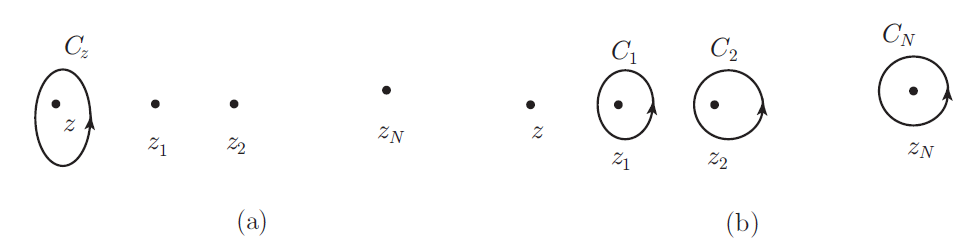
\includegraphics[width=0.6\linewidth]{fig/4.1.png}
	\caption{ (a)围绕$z$的闭合曲线,(b)围绕$z_1, \cdots, z_N$的闭合曲线。}
\end{figure}

右边用 $T(\zeta)$ 和 $\phi_i(z_i)$ 的OPE写成
\begin{equation}
	-\sum_{i=1}^{N} \int_{C_{i}} \frac{d \zeta}{2 \pi i}(\zeta-z)^{1-n}\left(\frac{h_{i}}{\left(\zeta-z_{i}\right)^{2}}+\frac{1}{\zeta-z_{i}} \partial_{i}\right)\left\langle\phi(z) \phi_{1}\left(z_{1}\right) \cdots \phi_{N}\left(z_{N}\right)\right\rangle
\end{equation}
计算$ \zeta=z_i $处的留数,得到
\begin{equation}
	\left\langle\left(L_{-n} \phi\right)(z) \phi_{1}\left(z_{1}\right) \cdots \phi_{N}\left(z_{N}\right)\right\rangle=\mathcal{L}_{-n}\left\langle\phi(z) \phi_{1}\left(z_{1}\right) \cdots \phi_{N}\left(z_{N}\right)\right\rangle
\end{equation}
其中
\begin{equation}
	\mathcal{L}_{-n}=\sum_{i=1}^{N}\left[\frac{(n-1) h_{i}}{\left(z_{i}-z\right)^{n}}-\frac{1}{\left(z_{i}-z\right)^{n-1}} \partial_{i}\right]
\end{equation}
重复这样的操作可得到
\begin{equation}
	\left\langle\left(L_{-n_{1}} \cdots L_{-n_{k}} \phi\right)(z) \phi_{1}\left(z_{1}\right) \cdots \phi_{N}\left(z_{N}\right)\right\rangle = \mathcal{L}_{-n_{1}} \cdots \mathcal{L}_{-n_{k}}\left\langle\phi(z) \phi_{1}\left(z_{1}\right) \cdots \phi_{N}\left(z_{N}\right)\right\rangle
\end{equation}
这样,计算包含次级场的关联函数,就转换成计算只包含初级场的关联函数。

\section{OPE的自举}
在共形场论中,Virasoro代数作用在局域场的空间上,初级场的共形类中的元素同Virasoro代数的Verma模中的元素一一对应。这个场的空间记作 $\mathcal{A}$ ,$ \mathcal{A}$ 是Virasoro代数的可约表示。将 $\mathcal{A} $分解成Virasoro代数的不可约表示,各不可约表示中有一个最高权向量,对应一个初级场。因此,局域场的空间 $\mathcal{A} $是初级场的共形类的直和,可分解成
$$
\mathcal{A}=\oplus_{\ell}\left[\phi_{\ell}\right]
$$
指标 $\ell$ 或离散,或连续。

场论中一个重要想法是自举(bootstrap)。这是由Polyakov\footnote{A. M. Polyakov, Sov. Phys. JETP 30 (1970) 151.},Kadanoff\footnote{L. P. Kadanoff, Phys. Rev. Lett. 23 (1969) 1430.}和Wilson\footnote{K. G. Wilson, Phys. Rev. 179 (1969) 1499.}提出的,同时提出的还有算符乘积展开和重整化群的想法。这一想法下,定义关联函数不是通过基本场 $\varphi(x) $的路径积分,而是通过$ \varphi(x) $和它的(包含导数的)复合场$ \varphi^{n_{0}}(\partial \varphi)^{n_{1}} \cdots$ 整体组成的局域场$ A_i(x) $的关联函数间的关系。局域场全体构成的空间 $\mathcal{A}$ 是完备集,也就是说,任何局域场都可写成 $\mathcal{A}$ 的基$ A_i(x)$ 的线性组合。那么,局域场 $A_i(x) $和 $A_j(y) $的算符乘积,就可在两点 $x,y$ 趋近时用 $\mathcal{A}$ 中的元素展开成
$$
A_{i}(x) A_{j}(y)=\sum_{k} C_{i j}^{k}(x, y) A_{k}(y)
$$
在二维共形场论中,初级场的共形类构成了局域场的完备集。可对初级场 $\phi_1(z,\bar{z})$ 和 $\phi_2(0,0)$ 的OPE作共形类分解:
\begin{equation}
	\phi_{1}(z, \bar{z}) \phi_{2}(0,0)=\sum_{k} C_{12}^{k} z^{-h_{1}-h_{2}+h_{k}} \bar{z}^{-\bar{h}_{1}-\bar{h}_{2}+\bar{h}_{k}} \Psi_{k}(z, \bar{z})
\end{equation}
这里,$ C_{12}^{k} $是常数,$ \Psi_{k}(z, \bar{z}) $可用共形类$ [\phi_k] $中的元素展开成
\begin{equation}
	\Psi_{k}(z, \bar{z})=\phi_{k}(0,0)+\beta_{1} z L_{-1} \phi_{k}(0,0)+\bar{\beta}_{1} \bar{z} \bar{L}_{-1} \phi_{k}(0,0)+\cdots
\end{equation}
这里作了归一化,以使$ \phi_{k}(0,0)$ 项的系数为1。因为Virasoro算符的右模 $L_{-n} $和左模$ \bar{L}_{-m}$ 独立地作用, $\Psi_{k}$ 对应的态 $|\Psi_{k}\rangle $可写成张量积
$$
\left|\Psi_{k}\right\rangle=\left|\psi_{k}\right\rangle \otimes |\bar{\psi}_{k} \rangle
$$
$\left|\psi_{k}\right\rangle$ 可展开成
\begin{equation}
	\left|\psi_{k}\right\rangle=\sum_{\{n\}} \beta_{12}^{k\{n\}} L_{-n_{1}} \cdots L_{-n_{p}}\left|\phi_{k}\right\rangle
\end{equation}
这里, $\{n\} $指非负整数的集合,其中的元素满足$ n_{1} \geq \cdots \geq n_{p}>0 $, $\beta_{12}^{k\{n\}} $是常数。相应地, $\Psi_{k}(z, \bar{z})$ 可写成
\begin{equation}
\begin{aligned} \Psi_{k}(z, \bar{z})=& \sum_{\{n\},\{m\}} \beta_{12}^{k\{n\}} \bar{\beta}_{12}^{k\{m\}} z^{\sum_{i} n_{i}} \bar{z}^{\sum_jm_{j}} \\ & \times L_{-n_{1}} \cdots L_{-n_{p}} \bar{L}_{-m_{1}} \cdots \bar{L}_{-m_{q}} \phi_{k}(0,0) \end{aligned}
\end{equation}
OPE (4.38) 作用在 $SL(2,\mathbb{C}) $不变真空$ |0\rangle$ 上,可以确定 $\beta,\bar{\beta} $:
\begin{equation}
	\phi_{1}(z, \bar{z}) \phi_{2}(0,0)|0\rangle=\sum_{k} C_{12}^{k} z^{-h_{1}-h_{2}+h_{k}} \bar{z}^{-\bar{h}_{1}-\bar{h}_{2}+\bar{h}_{k}}\left|\Psi_{k}(z, \bar{z})\right\rangle
\end{equation}
考虑$ L_n $( $n\geq 0 $)生成的无穷小共形变换。左边作用上$ L_n $得到
\begin{equation}
	L_{n}\left(\phi_{1}(z, \bar{z}) \phi_{2}(0,0)\right)|0\rangle=\left(\left[L_{n}, \phi_{1}(z, \bar{z})\right] \phi_{2}(0,0)+\phi_{1}(z, \bar{z})\left[L_{n}, \phi_{2}(0,0)\right]\right)|0\rangle
\end{equation}
因为$ L_n $对 $\phi_i(z,\bar{z}) $( $i=1,2 $)生成的无穷小变换是
\begin{equation}
	\left[L_{n}, \phi_{i}(z, \bar{z})\right]=z^{n+1} \partial \phi_{i}(z, \bar{z})+h_{i}(n+1) z^{n} \phi_{i}(z, \bar{z})
\end{equation}
$n>0$ 时有
\begin{equation}
L_{n}\left(\phi_{1}(z, \bar{z}) \phi_{2}(0,0)\right)|0\rangle=\left(\left(z^{n+1} \partial_{z}+h_{1}(n+1) z^{n}\right) \phi_{1}(z, \bar{z})\right) \phi_{2}(0,0)|0\rangle	
\end{equation}
$n=0 $时有
\begin{equation}
L_{0}\left(\phi_{1}(z, \bar{z}) \phi_{2}(0,0)\right)|0\rangle=\left(z \partial_{z}+h_{1}+h_{2}\right) \phi_{1}(z, \bar{z}) \phi_{2}(0,0)|0\rangle	
\end{equation}
由此知道 $|\psi_k\rangle$ 满足
\begin{align}
	L_{n} z^{-h_{1}-h_{2}+h_{k}}\left|\psi_{k}\right\rangle=&\left(z^{n+1} \partial_{z}+(n+1) h_{1} z^{n}\right) z^{-h_{1}-h_{2}+h_{k}}\left|\psi_{k}\right\rangle, \quad n>0,\\ L_{0} z^{-h_{1}-h_{2}+h_{k}}\left|\psi_{k}\right\rangle=&\left(z \partial_{z}+h_{1}+h_{2}\right) z^{-h_{1}-h_{2}+h_{k}}\left|\psi_{k}\right\rangle 
\end{align}
$|\psi_k\rangle$ 可展开成
\begin{equation}
	\left|\psi_{k}\right\rangle=\sum_{N=0}^{\infty} z^{N}\left|h_{k}, N\right\rangle
\end{equation}
例如
\begin{align} \left|h_{k}, 0\right\rangle &=\left|h_{k}\right\rangle &(4.50)\\ \left|h_{k}, 1\right\rangle &=\beta_{12}^{k\{1\}} L_{-1}\left|h_{k}\right\rangle \\ \left|h_{k}, 2\right\rangle &=\left(\beta_{12}^{k\{1,1\}} L_{-1}^{2}+\beta_{12}^{k\{2\}} L_{-2}\right)\left|h_{k}\right\rangle  \end{align}
(4.49) 代入 (4.47),(4.48) 。代入 (4.48) 得到的式子显然成立。代入 (4.47) 得到
\begin{equation}
	L_{n}\left|\psi_{k}\right\rangle=\sum_{N=0}^{\infty} z^{n+N}\left(N-h_{1}-h_{2}+h_{k}+(n+1) h_{1}\right)\left|h_{k}, N\right\rangle
\end{equation}
由此知道$ |h_k,N\rangle $满足
\begin{equation}
	L_{n}\left|h_{k}, N+n\right\rangle=\left(N+n h_{1}-h_{2}+h_{k}\right)\left|h_{k}, N\right\rangle
\end{equation}
于是可以看到,系数$ \beta_{12}^{k\{n\}}$ 可以递归地确定,并表示成中心荷$ c $和共形权的函数。

我们来具体确定低阶的 $\beta_{12}^{k\{n\}}$ 。 $n=1,N=0$ 时有
\begin{equation}
L_{1}\left|h_{k}, 1\right\rangle=\left(h_{k}+h_{1}-h_{2}\right)\left|h_{k}\right\rangle 
\end{equation}
进而得到
\begin{equation}
	2 h_{k} \beta_{12}^{k\{1\}}=h_{k}+h_{1}-h_{2}
\end{equation}
$n=2,N=0 $和 $n=1,N=1$ 时则可得到
\begin{equation}
\left(\begin{array}{cc} 2\left(2 h_{k}+1\right) & 3 \\ 6 h_{k} & 4 h_{k}+\frac{c}{2} \end{array}\right)\left(\begin{array}{c} \beta_{12}^{k\{1,1\}} \\ \beta_{12}^{k\{2\}} \end{array}\right)=\left(\begin{array}{c} \left(h_{k}+h_{1}-h_{2}+1\right) \beta_{12}^{k\{1\}} \\ h_{k}+2 h_{1}-h_{2} \end{array}\right)
\end{equation}

对一般的 $c,h_k $,上式左边的矩阵是可逆的, $\beta_{12}^{k\{1,1\}},\beta_{12}^{k\{2\}} $被唯一确定。然而,有些特殊情形下,矩阵不可逆,下章再说。

\section{交叉对称性}
上节说到,初级场$ \phi_1,\phi_2$ 的OPE中 $\Psi_k$ 的结构,可通过作无穷小共形变换来确定。但前面的系数 $C_{12}^k$ ,并不能从Virasoro代数的作用确定。如果要求初级场的OPE代数满足结合律 $\left(A_{i} A_{j}\right) A_{k}=A_{i}\left(A_{j} A_{k}\right) $,可以得到$ C_{ij}^k$ 满足的非线性条件。这说明,初级场的四点函数具有某种对称性(交叉对称性)。

考虑初级场的四点函数
\begin{equation}
	\left\langle\phi_{1}\left(z_{1}, \bar{z}_{1}\right) \phi_{2}\left(z_{2}, \bar{z}_{2}\right) \phi_{3}\left(z_{3}, \bar{z}_{3}\right) \phi_{4}\left(z_{4}, \bar{z}_{4}\right)\right\rangle
\end{equation}
全局的$ SL(2,\mathbb{C}) $共形变换,可用于固定初级场4个位置 $z_1,z_2,z_3,z_4 $中的3个。例如,作共形变换
\begin{equation}
	w=\frac{\left(z_{2}-z_{1}\right)\left(z-z_{4}\right)}{\left(z_{2}-z_{4}\right)\left(z-z_{1}\right)}
\end{equation}
这将点 $(z_1,z_2,z_3,z_4)$ 映到$ (\infty,1,x,0) $,其中
\begin{equation}
x=\frac{z_{21}z_{ 34}}{z_{24} z_{31}}
\end{equation}
是交比, $z_{ij}=z_i-z_j $。关联函数按Ward恒等式 (3.3) 变换。导数是
\begin{equation}
\frac{d w}{d z}=\frac{z_{21} z_{41}}{z_{24}} \frac{1}{\left(z-z_{1}\right)^{2}}
\end{equation}
在 $z=z_2,z_3,z_4$ 处分别是
\begin{equation}
	\begin{aligned} \left.\frac{d w}{d z}\right|_{z=z_{2}} & =\frac{z_{41}}{z_{24} z_{21}} \\ \left.\frac{d w}{d z}\right|_{z=z_{3}} & =\frac{z_{21} z_{41}}{z_{24} z_{31}^{2}} \\ \left.\frac{d w}{d z}\right|_{z=z_{4}} & =\frac{z_{21}}{z_{24} z_{41}} \end{aligned}
\end{equation}
$z=z_1$ 处是发散的,不过可以考虑取极限 $z=z_1'\to z_1 $,我们有
\begin{equation}
	\left.\frac{d w}{d z}\right|_{z=z_{1}^{\prime}}=\frac{z_{21} z_{41}}{z_{24}} \frac{1}{\left(z_{1}^{\prime}-z_{1}\right)^{2}} \sim \frac{z_{24}}{z_{21} z_{41}}\left(w_{1}^{\prime}\right)^{2}
\end{equation}
其中$w_1' $是 $z=z_1'$ 处 $w$ 的值。因此四点函数可写成
\begin{equation}
	\begin{aligned} &\left\langle\phi_{1}\left(z_{1}, \bar{z}_{1}\right) \phi_{2}\left(z_{2}, \bar{z}_{2}\right) \phi_{3}\left(z_{3}, \bar{z}_{3}\right) \phi_{4}\left(z_{4}, \bar{z}_{4}\right)\right\rangle \\ =&\left(\frac{z_{24}}{z_{21} z_{41}}\right)^{h_{1}}\left(\frac{z_{41}}{z_{24} z_{21}}\right)^{h_{2}}\left(\frac{z_{21} z_{41}}{z_{24} z_{31}^{2}}\right)^{h_{3}}\left(\frac{z_{21}}{z_{24} z_{41}}\right)^{h_{4}} \\ &\times\left(\frac{\bar{z}_{24}}{\bar{z}_{21} \bar{z}_{41}}\right)^{\bar{h}_{1}}\left(\frac{\bar{z}_{41}}{\bar{z}_{24} \bar{z}_{21}}\right)^{\bar{h}_{2}}\left(\frac{\bar{z}_{21} \bar{z}_{41}}{\bar{z}_{24} \bar{z}_{31}^{2}}\right)^{\bar{h}_{3}}\left(\frac{\bar{z}_{21}}{\bar{z}_{24} \bar{z}_{41}}\right)^{\bar{h}_{4}} G^{21}_{43}(x, \bar{x}) \end{aligned}
\end{equation}
其中
\begin{equation}
	\begin{aligned} G_{43}^{21}(x, \bar{x}) &=\lim _{w_{1}', \bar{w}_{1}' \rightarrow \infty}\left(w_{1}^{\prime}\right)^{2 h_{1}}\left(\bar{w}_{1}^{\prime}\right)^{2 \bar{h}_{1}}\left\langle\phi_{1}\left(w_{1}^{\prime}, \bar{w}_{1}^{\prime}\right) \phi_{2}(1,1) \phi_{3}(x, \bar{x}) \phi_{4}(0,0)\right\rangle \\ &=\left\langle\phi_{1}(\infty, \infty) \phi_{2}(1,1) \phi_{3}(x, \bar{x}) \phi_{4}(0,0)\right\rangle \end{aligned}
\end{equation}
我们引入$ Y_{43}^{21}(x, \bar{x}) $:
\begin{equation}
	G_{43}^{21}(x, \bar{x})=x^{\frac{h}{3}-h_{3}-h_{4}}(1-x)^{\frac{h}{3}-h_{2}-h_{3}} \bar{x}^{\frac{\bar{h}}{3}-\bar{h}_{3}-\bar{h}_{4}}(1-\bar{x})^{\frac{\bar{h}}{3}-\bar{h}_{2}-\bar{h}_{3}} Y_{43}^{21}(x, \bar{x})
\end{equation}
这样,四点函数可写成简单的形式
\begin{equation}
	\left\langle\phi_{1}\left(z_{1}, \bar{z}_{1}\right) \phi_{2}\left(z_{2}, \bar{z}_{2}\right) \phi_{3}\left(z_{3}, \bar{z}_{3}\right) \phi_{4}\left(z_{4}, \bar{z}_{4}\right)\right\rangle=\prod_{i<j}\left(z_{i j}\right)^{\gamma_{i j}}\left(\bar{z}_{i j}\right)^{\bar{\gamma}_{i j}} Y_{43}^{21}(x, \bar{x})
\end{equation}
其中
\begin{equation}
	\begin{aligned} &\gamma_{i j}=\frac{h}{3}-h_{i}-h_{j}, \quad h=h_{1}+h_{2}+h_{3}+h_{4}\\ &\bar{\gamma}_{i j}=\frac{\bar{h}}{3}-\bar{h}_{i}-\bar{h}_{j}, \quad \bar{h}=\bar{h}_{1}+\bar{h}_{2}+\bar{h}_{3}+\bar{h}_{4} \end{aligned}
\end{equation}

考虑另一个 $SL(2,\mathbb{C}) $变换,我们在 $z_1,z_2,z_3,z_4$ 中选取不同于上面例子的3个点,映到$ 0,1,\infty $。例如$ z_1 $映到 $\infty$ , $z_2 $映到 0 , $z_4 $映到 1 ,也就是交换初级场 $\phi_2,\phi_4$ ,那么作变换
\begin{equation}
	w=\frac{\left(z_{4}-z_{1}\right)\left(z-z_{2}\right)}{\left(z_{4}-z_{2}\right)\left(z-z_{1}\right)}
\end{equation}
这时, $z=z_3 $处的值是
\begin{equation}
	w_{3}=\frac{z_{41} z_{32}}{z_{42} z_{31}}=1-x
\end{equation}
四点函数可写成
\begin{equation}
	\begin{aligned} &\left\langle\phi_{1}\left(z_{1}, \bar{z}_{1}\right) \phi_{2}\left(z_{2}, \bar{z}_{2}\right) \phi_{3}\left(z_{3}, \bar{z}_{3}\right) \phi_{4}\left(z_{4}, \bar{z}_{4}\right)\right\rangle \\ =&\left(\frac{z_{42}}{z_{41} z_{21}}\right)^{h_{1}}\left(\frac{z_{21}}{z_{42} z_{41}}\right)^{h_{4}}\left(\frac{z_{41} z_{21}}{z_{42} z_{31}^{2}}\right)^{h_{3}}\left(\frac{z_{41}}{z_{42} z_{21}}\right)^{h_{2}} \\ & \times\left(\frac{\bar{z}_{42}}{\bar{z}_{41} \bar{z}_{21}}\right)^{\bar{h}_{1}}\left(\frac{\bar{z}_{21}}{\bar{z}_{42} \bar{z}_{41}}\right)^{\bar{h}_{4}}\left(\frac{\bar{z}_{41} \bar{z}_{21}}{\bar{z}_{42} \bar{z}_{31}^{2}}\right)^{\bar{h}_{3}}\left(\frac{\bar{z}_{41}}{\bar{z}_{42} \bar{z}_{21}}\right)^{\bar{h}_{2}} G_{23}^{41}(1-x, 1-\bar{x}) \end{aligned}
\end{equation}
比对 (4.64),(4.71) 可知,差一个相位因子的意义上有
\begin{equation}
	G_{43}^{21}(x, \bar{x})=G_{23}^{41}(1-x, 1-\bar{x})
\end{equation}
再考虑 $z_1 $映到 0 , $z_2 $映到 1 , $z_4 $映到 $\infty$,那么作变换
\begin{equation}
	w=\frac{\left(z_{2}-z_{4}\right)\left(z-z_{1}\right)}{\left(z_{2}-z_{1}\right)\left(z-z_{4}\right)}
\end{equation}
这时$ z_3 $映到$ 1/x$ 。同理可得
\begin{equation}
	G_{43}^{21}(x, \bar{x})=x^{-2 h_{3}} \bar{x}^{-2 \bar{h}_{3}} G_{13}^{24}\left(1/x, 1/\bar{x}\right)
\end{equation}
关联函数 $G_{n m}^{l k}(x, \bar{x}) $间的关系 (4.72),(4.74) 是从四点函数的全局共形对称性推出的,这称为四点函数的\textbf{交叉对称性(crossing symmetry)}。

我们来用OPE计算$ G_{43}^{21}(x, \bar{x})$ 。代入 $\phi_3(x,\bar{x})$ 和 $\phi_4(0,0) $的OPE,得到
\begin{equation}
	G_{43}^{21}(x, \bar{x})=\sum_{p} C_{43}^{p} C_{12}^{p} A_{43}^{21}(p | x, \bar{x})
\end{equation}
其中
\begin{equation}
	A_{43}^{21}(p | x, \bar{x})=\left(C_{12}^{p}\right)^{-1} x^{h_{p}-h_{3}-h_{4}} \bar{x}^{\bar{h}_{p}-\bar{h}_{3}-\bar{h}_{4}}\left\langle\phi_{1}\left|\phi_{2}(1,1) \Psi_{p}(x, \bar{x})\right| 0\right\rangle
\end{equation}
$A_{43}^{21}(p | x, \bar{x}) $可进一步分解成
\begin{equation}
	A_{43}^{21}(p | x, \bar{x})=F_{43}^{21}(p| x) \bar{F}_{43}^{21}(p | \bar{x})
\end{equation}
其中
\begin{equation}
	F_{43}^{21}(p |x)=x^{h_{p}-h_{3}-h_{4}} \sum_{\{n\}} \beta_{43}^{p\{n\}}x^{\sum_{i=1}^{k} n_{i}} \frac{\left\langle\phi_{1}\left|\phi_{2}(1,1) L_{-n_{1}} \cdots L_{-n_{k}}\right| \phi_{p}\right\rangle}{\left\langle\phi_{1}\left|\phi_{2}(1,1)\right| \phi_{p}\right\rangle}
\end{equation}
因此,${43}^{21}(p |x)$ 是构造四点函数的基础材料,称为\textbf{共形块(conformal block)}。

交叉对称性 (4.72) 成为
\begin{equation}
	\sum_{p} C_{43}^{p} C_{12}^{p} F_{43}^{21}(p | x) \bar{F}_{43}^{21}(p | \bar{x})=\sum_{q} C_{32}^{p} C_{14}^{q} F_{32}^{41}(q | 1-x) \bar{F}_{32}^{41}(q | 1-\bar{x})
\end{equation}
如果算出共形块,这就给出OPE系数 $C_{n m}^{l} $和共形权 $h_i $的方程。通过求解它,可以考察CFT的关联函数。这个方程是非线性的,很难解,不过人们已经详细研究了极小模型的结构。
